\section{Embedded Peripherals}
\subsection{Timers and Event Counters}
\subsubsection{Timer Structure}
A Binary Counter Driven by a Periodic Signal.It is possible to cascade multiple counters\\
\vspace{1cm}
\begin{minipage}{9cm}
	\begin{itemize}
		\item Mux -> Clock Source selector
		\item Prescaler -> Clock frequency divider
		\item Counter -> n-bit binary counter
		\item Comparator -> compares Counter Output with Compare Register
	\end{itemize}
\end{minipage}
\begin{minipage}{10cm}
	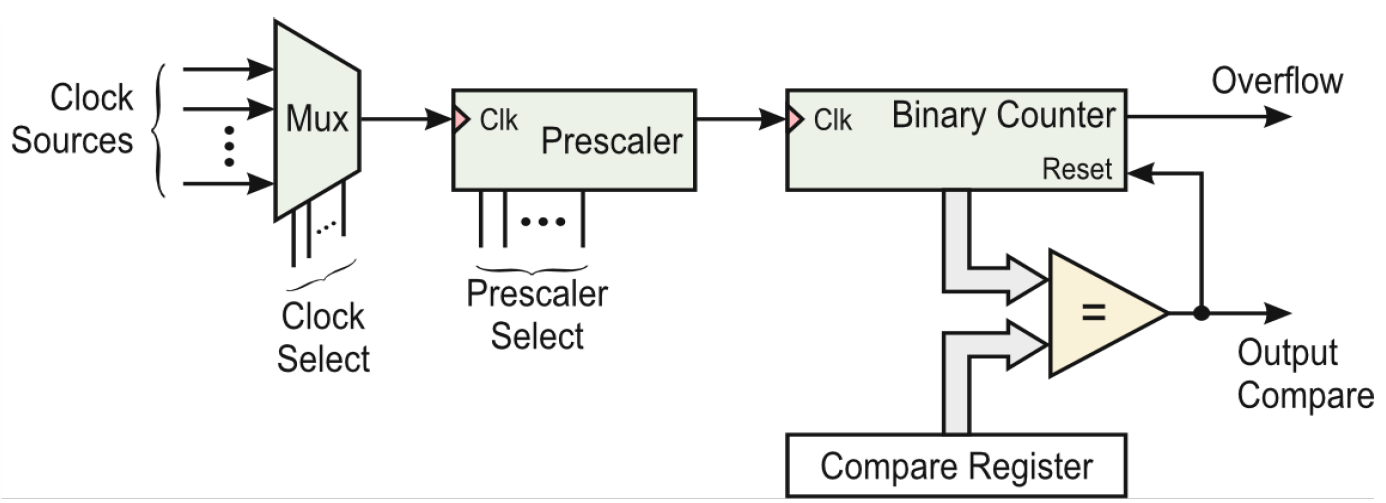
\includegraphics[width=10cm]{images/timerstructure.png} 
\end{minipage}
\begin{multicols}{2}
	\subsubsection{Interval Timer vs Event Counter}
	\begin{itemize}
		\item \textbf{Interval Timer}
		\subitem Measures the time elapsed after k clock cycles
		\item \textbf{Event Counter}
		\subitem Counts the occurrence of k external events
	\end{itemize}
	
	\subsubsection{Timer Application}
	\begin{itemize}
		\item Watchdog Timers (WDT)
		\item Realtime Clocks (RTC)
		\item Baud Rate Generator (BRG)
		\item Pulse-Width Modultation (PWM)
	\end{itemize}
\end{multicols}

\begin{tabular}{l l}
	\textbf{Watchdog Timer} & Monitor Events within an expiration intervals\\
	& If WDT expires before the event occurs, a default action is executed\\
	& If the event occurs within the defined interval, cancel and restart WDT\\
	& In MSP430 the WDT is 16-Bit (MaxCount: $2^{16}=32'768$) \\
	& and configure over Register WDTTMSEL\\
	\textbf{Realtime Clocks} &\\
	\textbf{Baud Rate Generator} & \\
	\textbf{Pulse-Width Modulation} & \\
	
\end{tabular}
\clearpage
\pagebreak